% questions.tex —— 2010 年·普通高等学校招生考试·湖北卷·文科 · 题目内容片段（无答案）
% 由 tools/generate_projects.py 依来源总账自 2010/2010_数学真题_湖北文_试题.md 生成，勿手改（改源 MD 后重跑）
状态：needs-review；依固定候选 PDF 两页（印刷页 599–600）逐题核验，三幅图已矢量重绘。原页未印分值，不补。

\gkpart{一、选择题}
\begin{question}
\gkti{1}设集合 $M=\{1,2,4,8\}$，$N=\{x\mid x\ \text{\text{是}}\ 2\ \text{\text{的倍数}}\}$，则 $M\cap N=$（　）

（A）$\{2,4\}$

（B）$\{1,2,4\}$

（C）$\{2,4,8\}$

（D）$\{1,2,4,8\}$

\end{question}
\begin{question}
\gkti{2}函数 $f(x)=\sqrt3\sin\left(\dfrac x2-\dfrac{\pi}{4}\right)$，$x\in\mathbf R$ 的最小正周期为（　）

（A）$\dfrac{\pi}{2}$

（B）$\pi$

（C）$2\pi$

（D）$4\pi$

\end{question}
\begin{question}
\gkti{3}已知函数 $f(x)=\begin{cases}\log_3 x,&x>0,\\2^x,&x\leqslant0,\end{cases}$ 则 $f\left(f\left(\dfrac19\right)\right)=$（　）

（A）$4$

（B）$\dfrac14$

（C）$-4$

（D）$-\dfrac14$

\end{question}
\begin{question}
\gkti{4}用 $a$、$b$、$c$ 表示三条不同的直线，$\gamma$ 表示平面，给出下列命题：

① 若 $a\parallel b$，$b\parallel c$，则 $a\parallel c$；

② 若 $a\perp b$，$b\perp c$，则 $a\perp c$；

③ 若 $a\parallel\gamma$，$b\parallel\gamma$，则 $a\parallel b$；

④ 若 $a\perp\gamma$，$b\perp\gamma$，则 $a\parallel b$。

正确的有（　）

（A）①②

（B）②③

（C）①④

（D）③④

\end{question}
\begin{question}
\gkti{5}函数 $y=\dfrac{1}{\sqrt{\log_{0.5}(4x-3)}}$ 的定义域为（　）

（A）$\left(\dfrac34,1\right)$

（B）$\left(\dfrac34,+\infty\right)$

（C）$(1,+\infty)$

（D）$\left(\dfrac34,1\right)\cup(1,+\infty)$

\end{question}
\begin{question}
\gkti{6}现有 6 名同学去听同时进行的 5 个课外知识讲座，每名同学可自由选择其中的一个讲座，不同选法的种数是（　）

（A）$5^6$

（B）$6^5$

（C）$\dfrac{5\times6\times5\times4\times3\times2}{2}$

（D）$6\times5\times4\times3\times2$

\end{question}
\begin{question}
\gkti{7}已知等比数列 $\{a_n\}$ 中，各项都是正数，且 $a_1$，$\dfrac12a_3$，$2a_2$ 成等差数列，则 $\dfrac{a_9+a_{10}}{a_7+a_8}=$（　）

（A）$1+\sqrt2$

（B）$1-\sqrt2$

（C）$3+2\sqrt2$

（D）$3-2\sqrt2$

\end{question}
\begin{question}
\gkti{8}已知 $\triangle ABC$ 和点 $M$ 满足 $\overrightarrow{MA}+\overrightarrow{MB}+\overrightarrow{MC}=\mathbf 0$。若存在实数 $m$ 使得 $\overrightarrow{AB}+\overrightarrow{AC}=m\overrightarrow{AM}$ 成立，则 $m=$（　）

（A）$2$

（B）$3$

（C）$4$

（D）$5$

\end{question}
\begin{question}
\gkti{9}若直线 $y=x+b$ 与曲线 $y=3-\sqrt{4x-x^2}$ 有公共点，则 $b$ 的取值范围是（　）

（A）$[1-2\sqrt2,1+2\sqrt2]$

（B）$[1-\sqrt2,3]$

（C）$[-1,1+2\sqrt2]$

（D）$[1-2\sqrt2,3]$

\end{question}
\begin{question}
\gkti{10}记实数 $x_1$，$x_2$，$\cdots$，$x_n$ 中的最大数为 $\max\{x_1,x_2,\cdots,x_n\}$，最小数为 $\min\{x_1,x_2,\cdots,x_n\}$。已知 $\triangle ABC$ 的三边边长为 $a$，$b$，$c$（$a\leqslant b\leqslant c$），定义它的倾斜度为 $t=\max\left\{\dfrac ab,\dfrac bc,\dfrac ca\right\}\cdot\min\left\{\dfrac ab,\dfrac bc,\dfrac ca\right\}$，则“$t=1$”是“$\triangle ABC$ 为等边三角形”的（　）

（A）必要而不充分的条件

（B）充分而不必要的条件

（C）充要条件

（D）既不充分也不必要的条件

\end{question}
\gkpart{二、填空题}
\begin{question}
\gkti{11}在 $(1-x^2)^{10}$ 的展开中，$x^4$ 的系数为 $\underline{\qquad}$。

\end{question}
\begin{question}
\gkti{12}已知 $z=2x-y$，式中变量 $x$，$y$ 满足约束条件 $\begin{cases}y\leqslant x,\\x+y\geqslant1,\\x\leqslant2,\end{cases}$ 则 $z$ 的最大值为 $\underline{\qquad}$。

\end{question}
\begin{question}
\gkti{13}一个病人服用某种新药后被治愈的概率为 $0.9$。则服用这种新药的 4 个病人中至少 3 人被治愈的概率为 $\underline{\qquad}$。（用数字作答）

\Needspace{0.4\textheight}
\end{question}
\begingroup
\renewenvironment{question}{\Needspace{0.5\textheight}}{}
\begin{question}
\gkti{14}圆柱形容器内部盛有高度为 $8\ \mathrm{cm}$ 的水，若放入三个相同的球（球的半径与圆柱的底面半径相同）后，水恰好淹没最上面的球（如图所示），则球的半径是 $\underline{\qquad}\ \mathrm{cm}$。
\nopagebreak[4]
\begin{center}% 2010 年湖北卷文科第 14 题：圆柱形容器内叠放三个相同小球的示意图。
% 来源 PDF：普通高考/2010/2010湖北文.pdf，SHA-256 70d7537f9072187051a41095e97fab1d72cc357ee9cd04e831da8cf99217af78。
% 原页：第 1 页（A3 三栏）第 2 栏中部，书页码 599。
% 重绘依据：照原页——容器以两条竖壁加浅灰底托表示；三个等球自上而下两两相切，
%   且都与柱壁相切（球半径等于底面半径）；柱口（顶部横线）恰在最上面一球的最高点，
%   即容器高度等于三个球的直径之和。球面用 ball 阴影表现明暗，不使用位图。
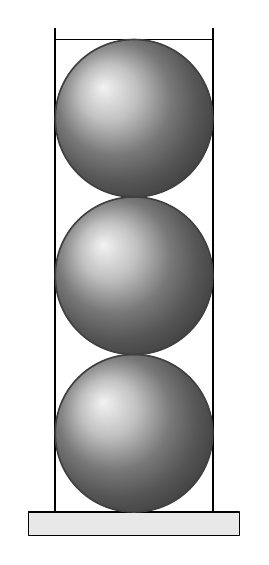
\begin{tikzpicture}[scale=1.0, semithick, line join=round]
  % 底托（浅灰扁矩形）
  \fill[gray!18] (-1.34,-0.30) rectangle (1.34,0);
  \draw (-1.34,-0.30) rectangle (1.34,0);
  % 柱壁（左右各一竖线，顶端略高出柱口，照原页）
  \draw (-1,0) -- (-1,6.14);
  \draw (1,0) -- (1,6.14);
  % 柱口：最上面一球的最高点处的横线
  \draw (-1,6) -- (1,6);
  % 三个球：半径 1，球心依次在 y=1,3,5（两两相切、与底和柱壁相切）
  \foreach \y in {1,3,5} {
    \shade[ball color=gray!65] (0,\y) circle (1);
    \draw[black!75] (0,\y) circle (1);
  }
\end{tikzpicture}
\end{center}
\nopagebreak[4]
\end{question}
\endgroup
\begin{question}
\gkti{15}已知椭圆 $C:\dfrac{x^2}{2}+y^2=1$ 的两焦点为 $F_1$，$F_2$，点 $P(x_0,y_0)$ 满足 $0<\dfrac{x_0^2}{2}+y_0^2<1$，则 $|PF_1|+|PF_2|$ 的取值范围为 $\underline{\qquad}$，直线 $\dfrac{x_0x}{2}+y_0y=1$ 与椭圆 $C$ 的公共点个数为 $\underline{\qquad}$。

\end{question}
\gkpart{三、解答题}
\begin{question}
\gkti{16}已经函数 $f(x)=\dfrac{\cos^2x-\sin^2x}{2}$，$g(x)=\dfrac12\sin2x-\dfrac14$。

（1）函数 $f(x)$ 的图象可由函数 $g(x)$ 的图象经过怎样变化得出？

（2）求函数 $h(x)=f(x)-g(x)$ 的最小值，并求使用 $h(x)$ 取得最小值的 $x$ 的集合。

\Needspace{0.4\textheight}
\end{question}
\begingroup
\renewenvironment{question}{\Needspace{0.5\textheight}}{}
\begin{question}
\gkti{17}为了了解一个小水库中养殖的鱼的有关情况，从这个水库中多个不同位置捕捞出 100 条鱼，称得每条鱼的质量（单位：千克），并将所得数据分组，画出频率分布直方图（如图所示）。
\nopagebreak[4]
\begin{center}% 2010 年湖北卷文科第 17 题：100 条鱼质量的频率分布直方图。
% 来源 PDF：普通高考/2010/2010湖北文.pdf，SHA-256 70d7537f9072187051a41095e97fab1d72cc357ee9cd04e831da8cf99217af78。
% 原页：第 1 页（A3 三栏）第 3 栏上部，书页码 599。
% 重绘依据：照原页——六个等宽组 [1.00,1.30)（组距 0.05），纵轴为「频率/组距」，
%   各矩形高依次为 0.4、1、4、5.6、6、3（矩形不加填充，故纵向虚线格线贯穿可见）；
%   纵轴刻度 0.4、1、3、4、5.6、6 处各引一条横向虚线指向对应矩形的顶边；
%   两轴均有断裂记号（横轴在 0 与 1.00 之间，纵轴贴近原点）。不代画任何数据。
\begin{tikzpicture}[x=1.5cm, y=0.72cm, semithick]
  % 坐标轴
  \draw[->, >=stealth] (0,0) -- (0,7.05);
  \draw[->, >=stealth] (-0.80,0) -- (6.95,0);
  % 轴断裂记号（横轴：0 与 1.00 之间；纵轴：贴近原点）
  \draw (-0.72,0.14) -- (-0.60,-0.14) -- (-0.48,0.14) -- (-0.36,-0.14);
  \draw (-0.09,0.08) -- (0.09,0.18);
  \draw (-0.09,0.24) -- (0.09,0.34);
  % 六个矩形（组距 0.05，高=频率/组距）
  \draw (0,0) rectangle (1,0.4);
  \draw (1,0) rectangle (2,1);
  \draw (2,0) rectangle (3,4);
  \draw (3,0) rectangle (4,5.6);
  \draw (4,0) rectangle (5,6);
  \draw (5,0) rectangle (6,3);
  % 纵轴刻度处的横向虚线：指向对应矩形的顶边
  % （0.4 一档即第一个矩形的顶边本身，不再另画）
  \draw[dashed, dash pattern=on 4pt off 3pt] (0,1) -- (1,1);
  \draw[dashed, dash pattern=on 4pt off 3pt] (0,3) -- (5,3);
  \draw[dashed, dash pattern=on 4pt off 3pt] (0,4) -- (2,4);
  \draw[dashed, dash pattern=on 4pt off 3pt] (0,5.6) -- (3,5.6);
  \draw[dashed, dash pattern=on 4pt off 3pt] (0,6) -- (4,6);
  % 纵轴刻度值
  \foreach \y/\v in {0.4/0.4, 1/1, 3/3, 4/4, 5.6/5.6, 6/6} {
    \node[anchor=east, inner sep=2pt] at (-0.16,\y) {$\v$};
  }
  % 横轴刻度值
  \node[anchor=north, inner sep=3pt] at (-0.72,-0.06) {$0$};
  \foreach \i/\v in {0/1.00, 1/1.05, 2/1.10, 3/1.15, 4/1.20, 5/1.25, 6/1.30} {
    \node[anchor=north, inner sep=3pt] at (\i,-0.06) {$\v$};
  }
  % 轴名
  \node[anchor=south, inner sep=1pt] at (-0.78,7.44) {频率};
  \draw (-1.30,7.14) -- (-0.26,7.14);
  \node[anchor=north, inner sep=1pt] at (-0.78,7.08) {组距};
  \node[anchor=west, inner sep=2pt] at (6.66,-0.34) {质量（$\mathrm{kg}$）};
\end{tikzpicture}
\end{center}
\nopagebreak[4]
（1）在下面表格中填写相应的频率；

\begin{center}
\begin{tabular}{ll}
\toprule
分组 & 频率 \\
\midrule
$[1.00,1.05)$ &  \\
$[1.05,1.10)$ &  \\
$[1.10,1.15)$ &  \\
$[1.15,1.20)$ &  \\
$[1.20,1.25)$ &  \\
$[1.25,1.30)$ &  \\
\bottomrule
\end{tabular}
\end{center}

（2）估计数据落在 $[1.15,1.30)$ 中的概率为多少；

（3）将上面捕捞的 100 条鱼分别作一记号后再放回水库，几天后再从水库的多处不同位置捕捞出 120 条鱼，其中带有记号的鱼有 6 条，请根据这一情况来估计该水库中鱼的总条数。

\Needspace{0.4\textheight}
\end{question}
\endgroup
\begingroup
\renewenvironment{question}{\Needspace{0.5\textheight}}{}
\begin{question}
\gkti{18}如图，在四面体 $ABOC$ 中，$OC\perp OA$，$OC\perp OB$，$\angle AOB=120^\circ$，且 $OA=OB=OC=1$。

（1）设 $P$ 为 $AC$ 的中点，$Q$ 在 $AB$ 上且 $AB=3AQ$，证明：$PQ\perp OA$；

（2）求二面角 $O-AC-B$ 的平面角的余弦值。
\nopagebreak[4]
\begin{center}% 2010 年湖北卷文科第 18 题：四面体 ABOC 及点 P、Q。
% 来源 PDF：普通高考/2010/2010湖北文.pdf，SHA-256 70d7537f9072187051a41095e97fab1d72cc357ee9cd04e831da8cf99217af78。
% 原页：第 2 页（A3 两栏）第 1 栏上部，书页码 600。
% 重绘依据：照原页——C 在最高处，B 在右，A 在左下，O 在形内偏下居中；
%   线段 CO、OA、OB 为虚线（被遮挡），CA、CB、AB 与 P Q 为实线；
%   P 在棱 CA 上（中点），Q 在棱 AB 上（AQ = AB/3），P Q 在图中穿过 CO、OA 两条虚线之间。
\begin{tikzpicture}[scale=0.78, semithick, line join=round]
  \coordinate (A) at (0,0);
  \coordinate (B) at (6.60,3.30);
  \coordinate (C) at (2.00,6.70);
  \coordinate (O) at (2.20,2.10);
  \coordinate (P) at ($(A)!0.5!(C)$);
  \coordinate (Q) at ($(A)!0.3333!(B)$);
  % 被遮挡的棱（虚线）
  \draw[dashed, dash pattern=on 4pt off 3pt] (C) -- (O);
  \draw[dashed, dash pattern=on 4pt off 3pt] (O) -- (A);
  \draw[dashed, dash pattern=on 4pt off 3pt] (O) -- (B);
  % 可见棱（实线）
  \draw (C) -- (A) -- (B) -- (C) -- cycle;
  % 截面内线段 P Q
  \draw (P) -- (Q);
  % 顶点与分点标注
  \node[above, inner sep=1pt] at (C) {$C$};
  \node[right, inner sep=1pt] at (B) {$B$};
  \node[below left, inner sep=1pt] at (A) {$A$};
  \node[right=2pt, inner sep=1pt] at (O) {$O$};
  \node[left=3pt, inner sep=1pt] at (P) {$P$};
  \node[below, inner sep=1pt] at (Q) {$Q$};
\end{tikzpicture}
\end{center}
\nopagebreak[4]
\end{question}
\endgroup
\begin{question}
\gkti{19}已知某地今年年初拥有居民住房的总面积为 $a$（单位：$\mathrm{m}^2$），其中有部分旧住房需要拆除。当地有关部门决定每年以当年年初住房面积的 $10\%$ 建设新住房，同时也拆除面积为 $b$（单位：$\mathrm{m}^2$）的旧住房。

（1）分别写出第一年末和第二年末的实际住房面积的表达式；

（2）如果第五年末该地的住房面积正好比今年年初的住房面积增加了 $30\%$，则每年拆除的旧住房面积 $b$ 是多少？（计算时取 $1.1^5=1.6$）

\end{question}
\begin{question}
\gkti{20}已知一条曲线 $C$ 在 $y$ 轴的右边，$C$ 上每一点到点 $F(1,0)$ 的距离减去它到 $y$ 轴距离的差都是 $1$。

（1）求曲线 $C$ 的方程；

（2）是否存在正数 $m$，对于过点 $M(m,0)$ 且与曲线 $C$ 有两个交点 $A$、$B$ 的任一直线，都有 $\overrightarrow{FA}\cdot\overrightarrow{FB}<0$？若存在，求出 $m$ 的取值范围；若不存在，请说明理由。

\end{question}
\begin{question}
\gkti{21}设函数 $f(x)=\dfrac13x^3-\dfrac a2x^2+bx+c$，其中 $a>0$，曲线 $y=f(x)$ 在点 $P(0,f(0))$ 处的切线方程为 $y=1$。

（1）确定 $b$，$c$ 的值；

（2）设曲线 $y=f(x)$ 在点 $(x_1,f(x_1))$ 及 $(x_2,f(x_2))$ 处的切线都过点 $(0,2)$。证明：当 $x_1\neq x_2$ 时，$f'(x_1)\neq f'(x_2)$；

（3）若过点 $(0,2)$ 可作曲线 $y=f(x)$ 的三条不同切线，求 $a$ 的取值范围。

\end{question}